
\section{Scalars and Vectors}
\begin{frame}
    \frametitle{Scalars vs Vectors}
    \begin{itemize}
        \item \textbf{Scalars:} Quantities described by a magnitude (e.g., temperature, mass).
        \item \textbf{Vectors:} Quantities described by both a magnitude and a direction (e.g., velocity, force).
    \end{itemize}
\end{frame}

\begin{frame}
    \frametitle{Vector Representation}
    \begin{itemize}
        \item Vectors can be represented graphically as arrows.
        \item The length of the arrow indicates the magnitude or it is shown as \(|\vec{v}|\).
        \item The direction of the arrow indicates the direction.
        \item Vectors are also denoted by a small arrow above the variable (e.g., \(\vec{v}\)).
    \end{itemize}
\end{frame}

\frame{
    \frametitle{Types of Vectors}
    \begin{itemize}
        \item \textbf{Zero Vector:} A vector with a magnitude of zero and no direction.
        \item \textbf{Unit Vector:} A vector with a magnitude of one, used to indicate direction and is given by \(\hat{v} = \frac{\vec{v}}{|\vec{v}|}\).
        \item \textbf{Position Vector:} A vector that represents the position of a point in space relative to an origin.
        \item \textbf{Collinear Vectors:} Vectors that lie along the same line or are parallel to each other.
        \item \textbf{Orthogonal Vectors:} Vectors that are perpendicular to each other.
        \item \textbf{Coplanar Vectors:} Vectors that lie in the same plane.
        \item \textbf{Negative Vectors:} Vectors that have the same magnitude as a given vector but point in the opposite direction.
        \item \textbf{Equal Vectors:} Vectors that have the same magnitude and direction.
        \item \textbf{Reciprocal Vectors:} Vectors having the same direction but their magnitudes are reciprocals of each other.
    \end{itemize}
}
\begin{frame}
    \frametitle{Position Vector}
    \begin{figure}
        \centering
        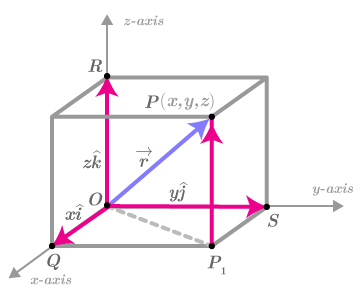
\includegraphics[width=0.4\textwidth]{scalars_vectors/position_vector.png}
        \caption{Position vector of a point in space}           
    \end{figure}
    
\end{frame}
\begin{frame}
    \frametitle{Position vector of a Point in Space}
    \begin{itemize}
        \item The position vector of a point \(P\) in space with coordinates \((x, y, z)\) is given by:
        \[
    \vec{OP} = x\hat{\imath} + y\hat{\jmath} + z\hat{k}
        \]
    where \(\hat{\imath}, \hat{\jmath}, \hat{k}\) are the unit vectors along the x, y, and z axes respectively. 

        \item The magnitude of the position vector is calculated as:
        \[
        |\vec{OP}| = \sqrt{x^2 + y^2 + z^2}
        \]
        \item The direction of the position vector is given by the angles it makes with the coordinate axes, which can be calculated using trigonometric functions.

    \end{itemize}
    
\end{frame}

\begin{frame}
    \frametitle{Direction Cosines}
    \begin{figure}
        \centering
        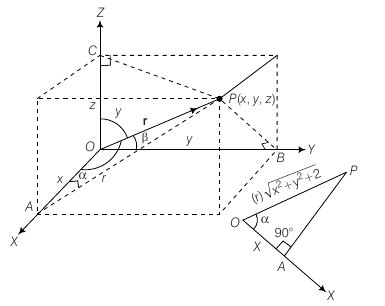
\includegraphics[width=0.6\textwidth]{scalars_vectors/direction_cosines.png}
        \caption{Direction cosines of a vector}
    \end{figure}
\end{frame}

\begin{frame}
    \frametitle{Direction Cosines}
    In $\delta OAP$ is right angled triangle 
    \[
    \cos \alpha = l = \frac{OA}{OP}  = \frac{x}{r} = \frac{x}{\sqrt{x^2 + y^2 + z^2}}
    \] 

    In $\delta OBP$ is right angled triangle
    \[
    \cos \beta = m = \frac{OB}{OP}  = \frac{y}{r} = \frac{y}{\sqrt{x^2 + y^2 + z^2}}
    \]

    In $\delta OCP$ is right angled triangle
    \[
    \cos \gamma = n = \frac{OC}{OP}  = \frac{z}{r} = \frac{z}{\sqrt{x^2 + y^2 + z^2}}
    \]
\end{frame}

\begin{frame}
    \frametitle{Direction Cosines}
    \begin{itemize}
        \item The direction cosines of a vector are the cosines of the angles that the vector makes with the coordinate axes.
        \item For a position vector \(\vec{OP}\), the direction cosines are given by:
        \[
        \cos \alpha = \frac{x}{|\vec{OP}|}, \quad \cos \beta = \frac{y}{|\vec{OP}|}, \quad \cos \gamma = \frac{z}{|\vec{OP}|}
        \]
        where \(\alpha, \beta, \gamma\) are the angles with the x, y, and z axes respectively.
        \item \(l^{2} + m^{2} + n^{2} = 1\)
    \end{itemize}
\end{frame}

\begin{frame}
    \frametitle{Direction Ratios}
    \begin{itemize}
        \item Direction ratios of \(\vec{OP}\) are any numbers proportional to \(x,y,z\); for the point \((x,y,z)\) itself they are \(x:y:z\).
        \item Relation with direction cosines: \(l=\frac{x}{r},\; m=\frac{y}{r},\; n=\frac{z}{r}\) where \(r=|\vec{OP}|=\sqrt{x^{2}+y^{2}+z^{2}}\); hence \(l:m:n = x:y:z\).
        \item Equivalently \(x = r l,\; y = r m,\; z = r n\). If you write \(l = kx,\; m = ky,\; n = kz\) then \(k = \tfrac{1}{r} = \tfrac{1}{|\vec{OP}|}\).
        \item In general, for any direction ratios \(a,b,c\): \(l = \frac{a}{\sqrt{a^{2}+b^{2}+c^{2}}},\; m = \frac{b}{\sqrt{a^{2}+b^{2}+c^{2}}},\; n = \frac{c}{\sqrt{a^{2}+b^{2}+c^{2}}}\).
    \end{itemize}
\end{frame}

\begin{frame}
\frametitle{Linear Combination of Vectors}
\begin{block}{Linear Combination}
A set of \(n\) vectors \(\vec{v_1}, \vec{v_2}, \ldots, \vec{v_n}\) can be combined linearly to form a new vector \(\vec{v}\):
\[
\vec{v} = c_1 \vec{v_1} + c_2 \vec{v_2} + \cdots + c_n \vec{v_n}
\]
where \(c_1, c_2, \ldots, c_n\) are scalars.
\end{block}
\end{frame}

\begin{frame}
    \frametitle{Relation between two Collinear Vectors}
    \begin{itemize}
        \item If two vectors \(\vec{a}\) and \(\vec{b}\) are collinear, then there exists a scalar \(k\) such that:
        \[
        \vec{b} = k \vec{a}
        \]
        where \(k\) is a non-zero scalar.
        \item Collinear vectors have the same or opposite direction.
        \item The scalar \(k\) can be positive or negative, indicating the direction of \(\vec{b}\) relative to \(\vec{a}\).
        \item If \(k > 0\), then \(\vec{b}\) points in the same direction as \(\vec{a}\). If \(k < 0\), then \(\vec{b}\) points in the opposite direction.
    \end{itemize}
\end{frame}

\begin{frame}
    \frametitle{Theorem of Coplanar Vectors}

    If three vectors \(\vec{a}, \vec{b}, \vec{c}\) are coplanar, then there exist scalars \(x, y, z\) such that:
    \[
    x \vec{a} + y \vec{b} + z \vec{c} = \vec{0}
    \]
    where not all of \(x, y, z\) are zero.      

    If two vectors \(\vec{a}, \vec{b}\) be two non-zero, non-collinear vectors, then any vector \(\vec{r}\) coplanar with \(\vec{a}\) and \(\vec{b}\) can be uniquely expressed as a linear combination of \(\vec{a}\) and \(\vec{b}\):
    \[
    \vec{r} = \lambda_1 \vec{a} + \lambda_2 \vec{b}
    \]
    for some scalars \(\lambda_1, \lambda_2\).

\end{frame}

\begin{frame}
\frametitle{Linear Dependence and Independence}
\begin{itemize}
    \item A set of vectors \(\{\vec{v_1}, \vec{v_2}, \ldots, \vec{v_n}\}\) is said to be linearly dependent if there exist scalars \(c_1, c_2, \ldots, c_n\), not all zero, such that:
    \[
    c_1 \vec{v_1} + c_2 \vec{v_2} + \cdots + c_n \vec{v_n} = \vec{0}
    \]
    \item If no such scalars exist, the vectors are linearly independent.
    \item Geometrically, linearly dependent vectors lie in the same line or plane, while independent vectors do not.
\end{itemize}                   
\end{frame}

\begin{frame}
    \frametitle{Product of Two Vectors}
    \begin{block}{Scalar product or Dot product}
        The scalar product (or dot product) of two vectors \(\vec{a}\) and \(\vec{b}\) is defined as:
        \[
        \vec{a} \cdot \vec{b} = |\vec{a}| |\vec{b}| \cos \theta
        \]
        where \(\theta\) is the angle between the two vectors.
        
    \end{block}
\end{frame}

\begin{frame}
    \frametitle{Geometric Interpretation of Dot Product}
    \begin{figure}
        \centering
        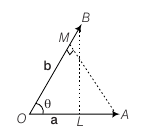
\includegraphics[width=0.4\textwidth]{scalars_vectors/dot_product.png}
        \caption{Geometric interpretation of the dot product}
    \end{figure}

\end{frame}

\begin{frame}
    \frametitle{Geometric Interpretation of Dot Product}
    From triangles \(\Delta OBL\) and \(\Delta OAM\):
    \begin{align*}
        OL &= OB \cos \theta \\
        OM &= OA \cos \theta  \\
        a \cdot b  &= |a| |b| \cos \theta = |a| proj_a b \\
        b \cdot a  &= |b| |a| \cos \theta = |b| proj_b a \\
    \end{align*}
\end{frame} 

\begin{frame}
\frametitle{Relevance of Dot Product: Physics}
The dot product is particularly useful in physics and engineering for calculating work done by a force. The work \(W\) done by a constant force \(\vec{F}\) acting on an object that undergoes a displacement \(\vec{d}\) is given by:
\[
W = \vec{F} \cdot \vec{d}
\]
\end{frame}

\begin{frame}
    \frametitle{Workdone by a Force}
    \begin{figure}
        \centering
        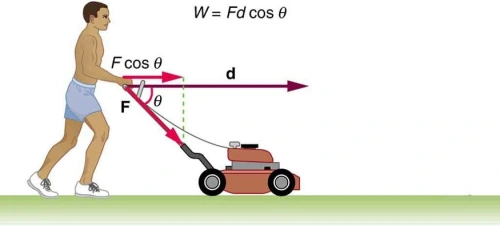
\includegraphics[width=0.8\linewidth]{scalars_vectors/force_dot.png}
    \end{figure}
\end{frame}

\begin{frame}
\frametitle{Force as a Scalar Product and the Role of Projection}
The work done by a force depends only on the component of the force in the direction of the displacement. If we write the unit vector in the direction of displacement as
\[
\hat{u}_{d} = \frac{\vec{d}}{|\vec{d}|},
\]
then the scalar (parallel) component of the force along the displacement is
\[
F_{\parallel} = \vec{F}\cdot\hat{u}_{d} = \frac{\vec{F}\cdot\vec{d}}{|\vec{d}|}.
\]
\end{frame} 

\begin{frame} 
    \frametitle{Force as a Scalar Product and the Role of Projection}
The work can therefore be written as the product of this scalar component and the magnitude of the displacement:
\[
W = F_{\parallel}\,|\vec{d}| = (\vec{F}\cdot\hat{u}_{d})\,|\vec{d}| = \vec{F}\cdot\vec{d}.
\]

The vector projection of \(\vec{F}\) onto \(\vec{d}\) (the part of the force that actually does the work) is
\[
\mathrm{proj}_{\vec{d}}\vec{F} = \left(\frac{\vec{F}\cdot\vec{d}}{|\vec{d}|^{2}}\right)\vec{d}.
\]
\end{frame} 

\begin{frame} 
    \frametitle{Workdone by a Force}
Key points:
\begin{itemize}
    \item Only the component of \(\vec{F}\) parallel to the displacement contributes to work; the perpendicular component does no work because its dot product with \(\vec{d}\) is zero.
    \item Writing work in terms of the projection makes the physical meaning clear: you are multiplying the displacement by the effective force acting along that displacement.
    \item Example: if an object is displaced horizontally by \(\vec{d}=d\hat{\imath}\) and \(\vec{F}=(F_x,F_y)\), then \(W=F_x d\) — only the horizontal component contributes.
\end{itemize}
\end{frame}
\begin{frame}
\frametitle{Relevance of Dot Product: Mathematics and Computer Science}
The dot product is also important in mathematics and computer science. Its applications include:
\begin{itemize}
    \item \textbf{Projection}: The dot product is used to project one vector onto another, which is useful in various algorithms.
    \item \textbf{Similarity}: In machine learning, the dot product is used to measure the similarity between two vectors, such as in document classification.
    \item \textbf{Graphics}: The dot product helps in determining the angle between vectors, which is essential in computer graphics for lighting and shading calculations.
\end{itemize}
\end{frame}
\begin{frame}
    \frametitle{Algebraic Properties of Dot Product}
    \begin{itemize}
        \item Commutative: \(a \cdot b = b \cdot a\)
        \item Distributive: \(a \cdot (b + c) = a \cdot b + a \cdot c\)
        \item Scalar multiplication: \((k a) \cdot b = k (a \cdot b)\)
    \end{itemize}
\end{frame}

\begin{frame}
    \frametitle{Vector Product or Cross Product}
    The vector product (or cross product) of two vectors \(\vec{a}\) and \(\vec{b}\) is defined as:
    \[
    \vec{a} \times \vec{b} = |\vec{a}| |\vec{b}| \sin \theta \, \hat{n}
    \]
    where \(\theta\) is the angle between the two vectors and \(\hat{n}\) is a unit vector perpendicular to the plane containing \(\vec{a}\) and \(\vec{b}\), following the right-hand rule.
\end{frame}

\begin{frame}
\frametitle{Geometric Interpretation of Cross Product}
\begin{figure}
    \centering
    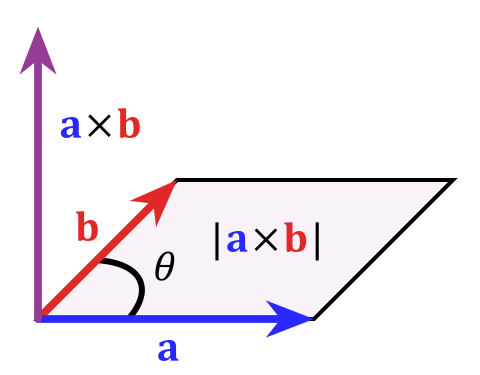
\includegraphics[width=0.4\textwidth]{scalars_vectors/cross_product.png}
    \caption{Geometric interpretation of the cross product}
\end{figure}
\end{frame} 

\begin{frame}
    \frametitle{Geometric Interpretation of Cross Product}
    The area of a parallelogram formed by two vectors \(\vec{a}\) and \(\vec{b}\) is given by the magnitude of their cross product:
    \[
    A = |\vec{a} \times \vec{b}|
    \]
    where \(\theta\) is the angle between the two vectors.

\end{frame}

\begin{frame}
    \frametitle{Algebraic Properties of Cross Product}
    \begin{itemize}
        \item Anticommutative: \(\vec{a} \times \vec{b} = -(\vec{b} \times \vec{a})\)
        \item Distributive: \(\vec{a} \times (\vec{b} + \vec{c}) = \vec{a} \times \vec{b} + \vec{a} \times \vec{c}\)
        \item Scalar multiplication: \((k \vec{a}) \times \vec{b} = k (\vec{a} \times \vec{b})\)
        \item The cross product of two parallel vectors is zero: if \(\vec{a}\) and \(\vec{b}\) are parallel, then \(\vec{a} \times \vec{b} = 0\).
        \item The magnitude of the cross product can be interpreted as the area of the parallelogram formed by the two vectors: \(|\vec{a} \times \vec{b}| = |\vec{a}| |\vec{b}| \sin \theta\).
    \end{itemize}
\end{frame}

\begin{frame}
    \frametitle{Relevance of Cross Product: Physics}
    The cross product is particularly useful in physics and engineering for determining a vector that is perpendicular to a plane defined by two other vectors. This has applications in:
    \begin{itemize}
        \item \textbf{Torque}: The torque \(\vec{\tau}\) exerted by a force \(\vec{F}\) applied at a position \(\vec{r}\) is given by the cross product:
        \[
        \vec{\tau} = \vec{r} \times \vec{F}
        \]
        \item \textbf{Angular Momentum}: The angular momentum \(\vec{L}\) of a particle is given by:
        \[
        \vec{L} = \vec{r} \times \vec{p}
        \]
        where \(\vec{p}\) is the linear momentum.
        \item \textbf{Magnetic Force}: The force \(\vec{F}\) on a charged particle moving with velocity \(\vec{v}\) in a magnetic field \(\vec{B}\) is given by:
        \[
        \vec{F} = q \vec{v} \times \vec{B}
        \]
    \end{itemize}
\end{frame}

\begin{frame}
    \frametitle{Force and Torque} 
    \begin{figure}
        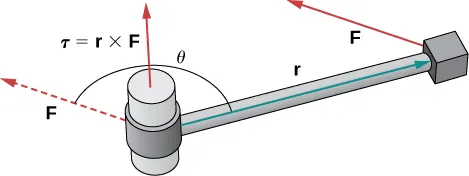
\includegraphics[width=0.8\linewidth]{scalars_vectors/torque_force.png}
    \end{figure}
\end{frame}

\begin{frame}
    \frametitle{Relevance of Cross Product: Mathematics and Computer Graphics}
    The cross product is also important in mathematics and computer graphics. Its applications include:
    \begin{itemize}
        \item \textbf{Normal Vectors}: In computer graphics, the cross product is used to find normal vectors to surfaces, which are essential for lighting calculations.
        \item \textbf{3D Rotations}: The cross product helps in determining the axis of rotation and the angle of rotation in 3D space.
        \item \textbf{Area Calculation}: The magnitude of the cross product of two vectors can be used to find the area of the parallelogram formed by the vectors.
    \end{itemize}
\end{frame}

\begin{frame}
    \frametitle{Algebraic properties of Vector Product}
    \begin{itemize}
        \item Anticommutative: \(\vec{a} \times \vec{b} = -(\vec{b} \times \vec{a})\)
        \item Distributive: \(\vec{a} \times (\vec{b} + \vec{c}) = \vec{a} \times \vec{b} + \vec{a} \times \vec{c}\)
        \item Scalar multiplication: \((k \vec{a}) \times \vec{b} = k (\vec{a} \times \vec{b})\)
        \item The cross product of two parallel vectors is zero: if \(\vec{a}\) and \(\vec{b}\) are parallel, then \(\vec{a} \times \vec{b} = 0\).
        \item The magnitude of the cross product can be interpreted as the area of the parallelogram formed by the two vectors: \(|\vec{a} \times \vec{b}| = |\vec{a}| |\vec{b}| \sin \theta\).
    \end{itemize}
\end{frame}

\begin{frame}
\frametitle{Vector Product in terms of Components}
The cross product of two vectors \(\vec{a} = (a_1, a_2, a_3)\) and \(\vec{b} = (b_1, b_2, b_3)\) can be expressed in terms of its components as follows:
\[
\vec{a} \times \vec{b} = \begin{vmatrix}
\hat{i} & \hat{j} & \hat{k} \\
a_1 & a_2 & a_3 \\
b_1 & b_2 & b_3
\end{vmatrix}
= \hat{i}(a_2b_3 - a_3b_2) - \hat{j}(a_1b_3 - a_3b_1) + \hat{k}(a_1b_2 - a_2b_1)
\]
\end{frame}

\begin{frame}
\frametitle{Vector Normal to the plane of Two given Vectors}
If \(\vec{a}\) and \(\vec{b}\) are two non-parallel, non-zero vectors in \(\mathbb{R}^3\) and let \(\theta\) be the angle between them, then 
\begin{align*}
    \vec{a} \times \vec{b} &= |\vec{a}| |\vec{b}| \sin \theta \, \hat{n} \\
    \hat{n} &= \frac{\vec{a} \times \vec{b}}{|\vec{a} \times \vec{b}|}
\end{align*}             
\end{frame}





